\documentclass[11pt]{article}
\usepackage{classTools}
\usepackage{tikz}

\draftfalse

\begin{document}

\psHeader{6}{Wed Oct. 26, 2022 (11:59pm)}

\textbf{Your name: Andrew Courtney}

\textbf{Collaborators: }

\textbf{No. of late days used on previous psets: 6}

\textbf{No. of late days used after including this pset: 3}

\begin{enumerate}
 \item (Matching Algorithms) 

 One practical application of matching algorithms is planning logistics, like in the following example from (fictional) ridesharing service Lyber in (real) New York City's Times Square.  When a customer books a Lyber ride, the ride request is sent to a Lyber server and combined with others to create a schematic 

 like the one drawn in the map below:


\begin{figure}[H]
    \centering
    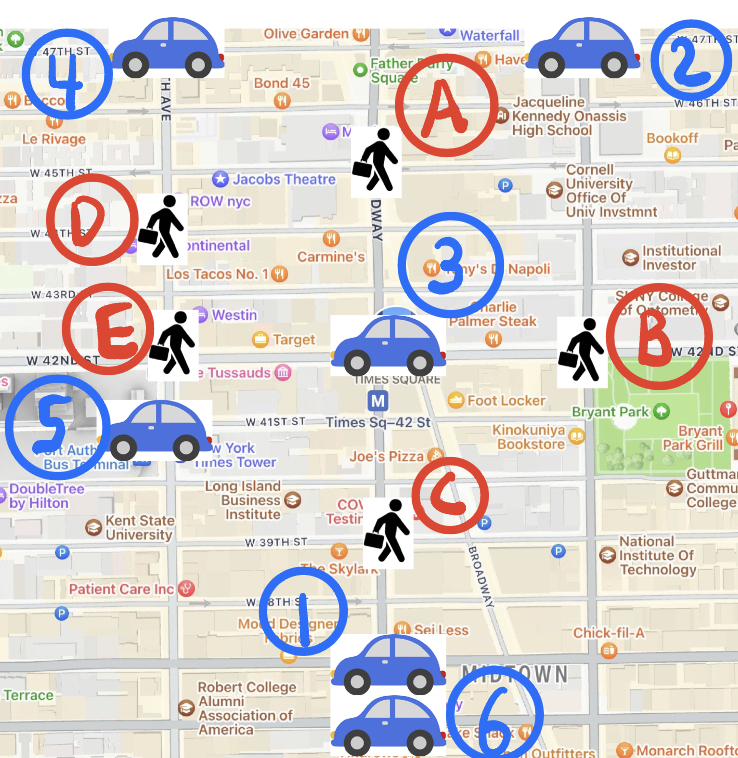
\includegraphics[width=0.87\textwidth]{NYC-map-zoomed-light.jpeg}
    \label{fig:travel_time_graph}
\end{figure}

Given a schematic like this, Lyber's goal is to serve as many customers (labeled A--E in the map) as possible, by assigning each one to a driver (labeled 1--6 in the map). For simplicity, each customer and driver is at an intersection, and assume driving between adjacent streets (vertical segment) takes 30 seconds, and driving between adjacent avenues (horizontal segments) takes 1 minute. However, the one twist is that they want to make sure that \textit{no customer is waiting for longer than 2 minutes}.  They also do not want to assign a driver to more than one customer at once, since serving a single customer can take more than 2 minutes.

    \begin{enumerate}
    \item To perform the assignment, they reduce to Maximum Matching in bipartite graphs.  Draw a bipartite graph corresponding to the drivers and customers in the map above.
    
\begin{proof}[Solution]
Here is the graph, with drivers on the top and customers on the bottom. \\
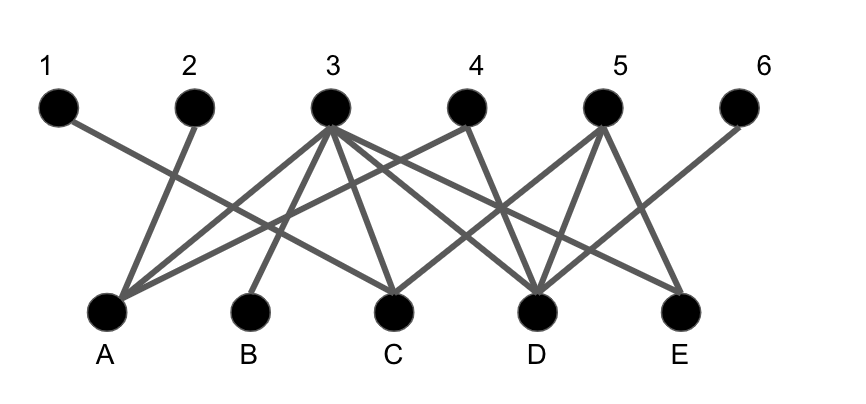
\includegraphics[width=4in]{1-1}
\end{proof}

    
    \item The Lyber app first prioritizes customers on Broadway, so they initially assign customer $A$ to driver 3 and customer $C$ to driver 5. Using the algorithm from class, find a \textit{maximum matching} in the bipartite matching graph you've drawn, starting from the initial matching of $A$ to 3 and $C$ to 5. Draw pictures showing the sequence of matchings and augmenting paths you find. (No need to break down the steps of the algorithm to find the augmenting paths.)

\begin{proof}
We walk through the graph, starting with $\{ A, 3 \}$ and $\{C, 5 \}$ as matchings. Here, matchings are always labeled in orange, and augmented paths are always labeled in blue (before they're added to the graph permanently). \\
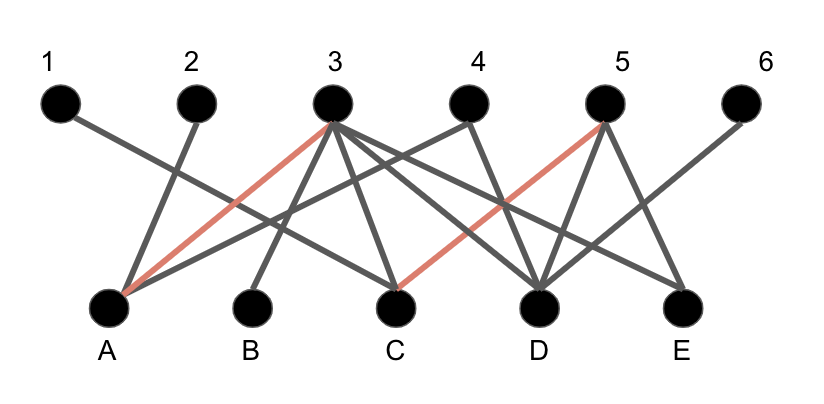
\includegraphics[width=4in]{1-2} \\
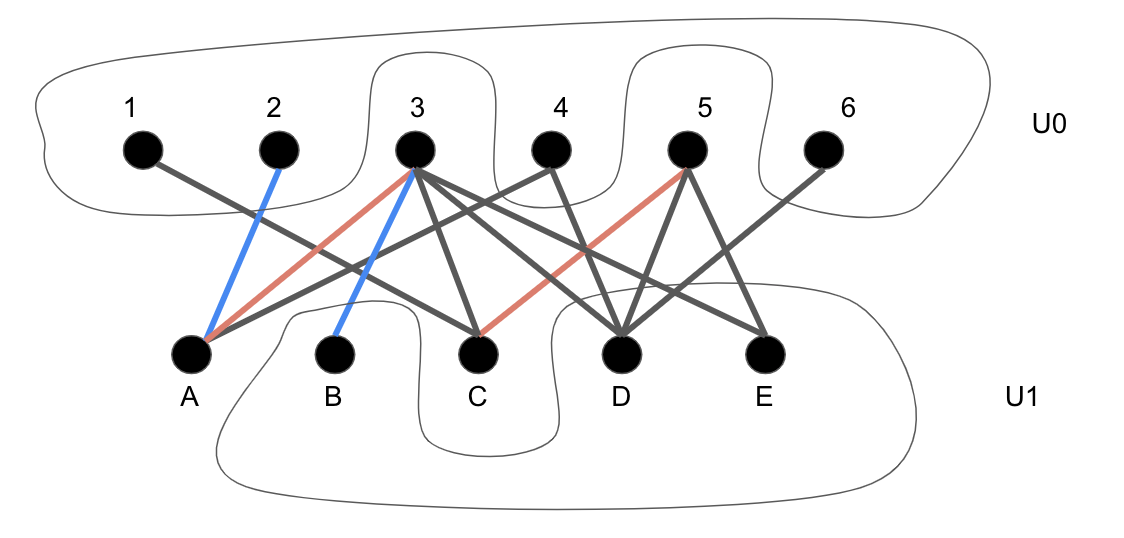
\includegraphics[width=4in]{1-3} \\
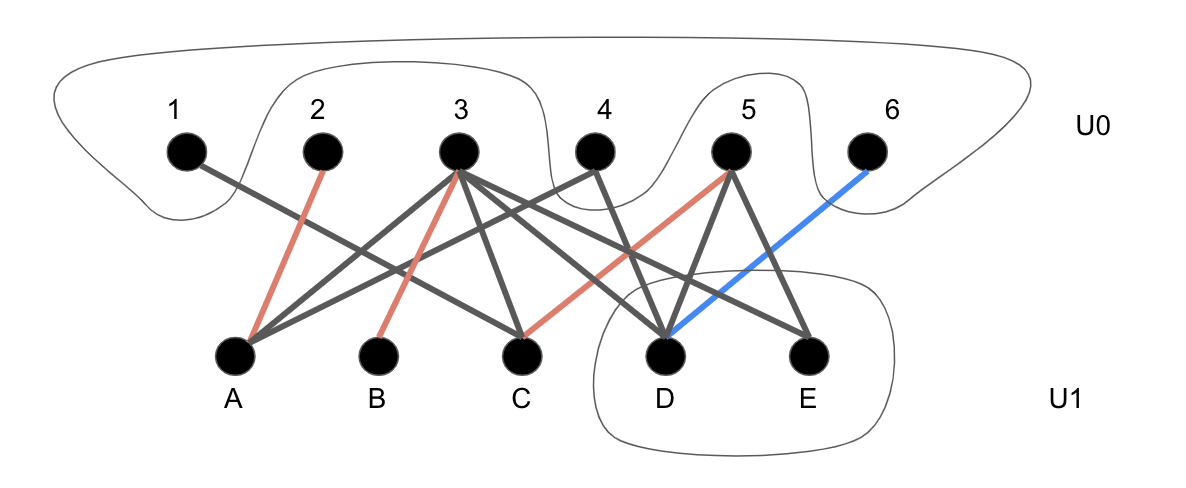
\includegraphics[width=4in]{1-4} \\
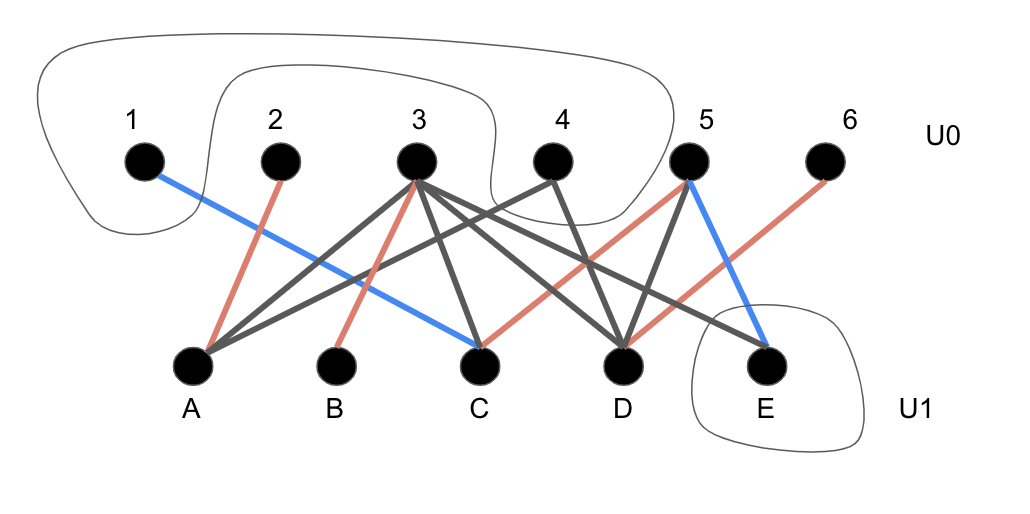
\includegraphics[width=4in]{1-5} \\
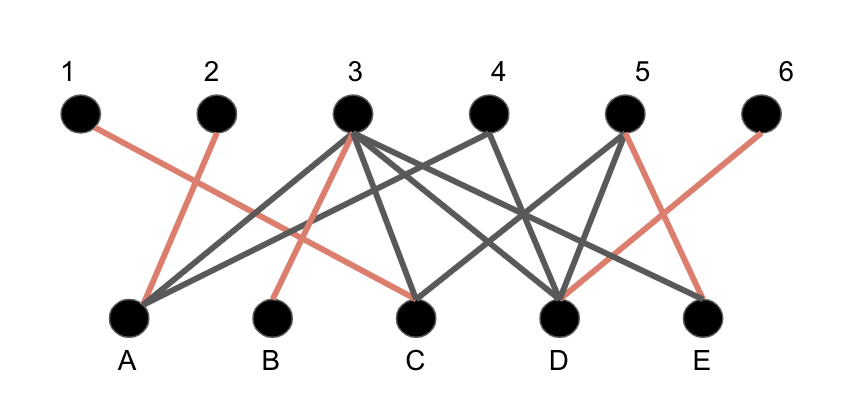
\includegraphics[width=4in]{1-6} \\

At the end, every passenger has a cab they can take.
\end{proof}

    \item The Lyber app also allows users to schedule trips in advance. One Lyber driver receives the following pre-programmed trips scheduled by 4 different users (all of them need multiple rides on the same day):
    \begin{itemize}
        \item User A: one trip from 10 to 10:29, another from 11 to 11:59, another from 12:15 to 12:29, and another from 13 to 13:29.
        \item User B: one trip from 10:15 to 11:14, another from 11:30 to 12:14, and another from 12:45 to 13:14.
        \item User C: one trip from 10:30 to 11:44, another from 12:30 to 12:59, and another from 13:15 to 13:44.
        \item User D: one trip from 10 to 10:44, another from 11:15 to 11:29, another from 12 to 12:44, and another from 13:30 to 13:59.
    \end{itemize}
    The Lyber driver wants to maximize the total number of different rides, because they earn a fixed rate per ride. (The driver is \textit{not} trying to maximize the driving time). 

    We also assume for simplicity that the driver needs no time to move between different rides (i.e., it is possible that one ride finishes at 10:29 and the next one starts immediately at 10:30). 

    Use a greedy algorithm that we saw in class to find a maximum-sized set of non-conflicting rides.  State which algorithm you are using, how you are applying it to this ride-selection problem, and write down the order in which the greedy algorithm selects the rides in the solution. 

\begin{proof}
We use the greedy interval scheduling algorithm, which we know from Theorem 2.3 in the Lecture 12 notes returns an optimal solution to the Interval Scheduling problem. The algorithm is quite simple - we sort all intervals $[a, b]$ in increasing order by the size of $b$, the endtime of the ride. For notational ease, we'll list every ride in the form $([a, b], C)$, where $[a, b]$ is the time of the trip and $C$ is the passenger. Here is how we sort it:

([10:00, 10:29], A), ([10:00, 10:44], D), ([10:15, 11:14], B), ([11:15, 11:29], D), ([10:30, 11:44], C), ([11:00, 11:59], A), ([11:30, 12:14], B), ([12:15, 12:29], A), ([12:00, 12:44], D), ([12:30, 12:59], C), ([12:45, 13:14], B), ([13:00, 13:29], A), ([13:15, 13:44], C), ([13:30, 13:59], D).

Then, sorting through the list and choosing elements which do not overlap greedily, we get the list of trips:

([10:00, 10:29], A), ([11:15, 11:29], D), ([11:30, 12:14], B), ([12:15, 12:29], A), ([12:30, 12:59], C),  ([13:00, 13:29], A), ([13:30, 13:59], D).

So the driver can give at most seven rides, and this is the list which the greedy interval scheduling algorithm selects.

\end{proof}

    \end{enumerate}

 \item (EthiCS Reflection) 
 Suppose there are two patients in need of an immediate kidney transplant, but only one donor is currently available. The donor'��s kidney is compatible with both patients. Patient A is 30 years old, and is expected to live 6 additional years as a result of the transplant. Patient B is 60 years old, and is expected to live 10 additional years as a result of the transplant. {\em All else being equal} (e.g., both patients have an urgent need for the transplant; both patients have been on the kidney exchange waiting list for the same length of time), \underline{\textbf{which patient should the kidney go to, and why?}} Your response should take the form of a short paragraph (3-4 sentence) reflection. {\em In explaining your ethical reasoning about the case, be sure to draw on at least one concept discussed in class.}
 
\begin{proof}[Response]

For me, the kidney should go to patient B. From a utilitarian point of view, this makes sense from both a first and second order review; the value of an extra four life-years is hard to beat; from a second order approach, it's hard to come up with a reason for why the 30-year-old would be more meaningful to those around them than the 60-year-old. I don't think you could make a productivity argument - I'm not sure that the 30-year-old being sickly and alive for another 6 years would contribute more to the GDP than the 60-year-old would over 10 years. The argument for the 30-year-old is that it would be ``fairer" for them to get more years of life because they've had less, which I understand - but I'd rather see that as a tiebreaker than something that makes a difference when four years hangs in the difference.

\end{proof}

 \item (Vertex-Weighted Matching)
        For a graph $G=(V,E)$ and a subset $F\subseteq E$, 

        let $V(F)$ denote the set $\bigcup_{f \in F}f$ of 
        vertices that are an endpoint of at least one edge in $F$.
        \begin{enumerate}
        \item \label{part:monotonicity} Prove that if $G=(V,E)$ is a graph and $M\subseteq E$ is a matching in $G$, then there is a maximum-size matching $M'$ such that $V(M)\subseteq V(M')$.  (Hint: consider constructing a maximum matching via augmenting paths, but starting with $M_0=M$ rather than $M_0=\emptyset$. What can you say about the $V(M_i)$'s?)
        
\begin{proof}
We use Berge's Theorem from the Lecture 13 notes. Berge's Theorem tells us that if $M$ is a matching of a graph $G$ which is not a maximum-size matching, then $G$ has an augmenting path with respect to $M$. Then we can apply this to the situation. 

Suppose $M_0$ is a matching in $G$. If $M_0$ is a maximum-size matching, then clearly the condition is satisfied. Suppose $M_0$ is not a maximum-size matching. Then we can use Berge's Theorem to construct an augmented path in $M_0$ and return some new $M_1$, which contains all of the nodes of $M_0$ and two additional nodes (by the definition of augmented path). We continue this algorithm until $M_n$ is a maximum-size matching for some $n$; this must exist because we can apply this algorithm at most $k/2$ times if there are $k$ nodes in the graph, so the algorithm terminates. Then $M_n$ contains every single node that $M_0$ has, because every $M_{i+1}$ has all the nodes of $M_{i}$ (this is obvious inductively). Therefore $V(M_0) \subseteq V(M')$, which is what we desired.
\end{proof}

        \item   In the Embedded EthiCS module, we saw how simply maximizing the {\em size} of a matching may not always be the right objective.  Thus, it is natural to consider weighted versions of the matching problem. Suppose we
        we consider vertex-weighted graphs $G = (V,E,w)$, $w$ is an array specifying a nonnegative edge weight $w(v)$ for every $v\in V$.  (For example, the weight assigned to a patient might correspond to the number of extra years of life they would gain from a donation.)
          The goal of the {\em vertex-weighted maximum matching problem} is to find a matching $M$ maximizing its {\em total weight} $$w(M) = \sum_{\{u,v\}\in M} (w(u)+w(v)).$$
        (This corresponds to the utilitarian objective discussed in Embedded EthiCS module.)
        Using Part~\ref{part:monotonicity}, prove that every graph $G$ has a matching $M^*$ that simultaneously maximizes both total weight and size.  That is, for every matching $M$ in $G$, we have
        both $w(M)\leq w(M^*)$ and $|M|\leq |M^*|$.

\begin{proof}
Suppose there is some $M$ which maximizes the weights but not size for the sake of contradiction. Then because weights have nonnegative values, we can apply ~\ref{part:monotonicity} to find some $M'$ which contains all the nodes of $M$ and is also of maximal size (and we are guaranteed this graph $M'$ exists). Because $w(M')$ cannot be less than $w(M)$ as all nodes have nonnegative value, $w(M) = w(M')$; also, $|M| < |M'|$, which means that this new graph is maximal in weights and size.
\end{proof}

        \item (optional\footnote{This problem won't make a difference between N, L, R-, and R grades. As this problem is purely extra credit, course staff will deprioritize questions about this problem at office hours and on Ed.}) Explain why the same holds for the maximin objective discussed in the Embedded EthiCS module.  That is, there is always a matching $M$ that simultaneously maximizes the maximin objective and $|M|$. 
        
\begin{proof}
We use the same principle here. The maximin objective asks that the solution found is the one which maximizes the weight given to the person who is least well off at the end of the action. This means that there is a hierarchy of nodes which we would like to include in our graph - some node that we want to include the most, some node we'd want the second most, and so on. Then our vertex-weighted graph $G = (V, E, w)$ would have weights $w$ which represent how badly we want to include each node in our final response, where 1 is the most important and $n = |V|$ is the least important. The optimal $M'$ is the one where the smallest weight not included in $M'$ is as large as possible.

So suppose $M'$ is optimized on the maximin objective but is not the largest possible size - that is, there is some smallest $i$ for which the node with $w = i$ is in $M'$ but the node with $w = i + 1$ is not, and this is the largest possible $i$ across all constructions of $M$. Then we can apply~\ref{part:monotonicity} over and over again, as in the previous part, to get some $M^*$ which contains all the nodes of $M'$ but is also of maximum size. If $w = i + 1$ is in $M^*$, this contradicts the assumption that $M'$ is optimized on the maximin objective; therefore, we have a graph of maximal size which has some smallest $i$ for which the node with $w = i$ is in $M^*$ but the node with $w = i + 1$ is not. Clearly, we have constructed an $M^*$ that optimizes on size and on the maximin objective, so we are done.
\end{proof}
        \end{enumerate}
        

\item (Edge-Weighted Bipartite Matching) 
  Instead of considering vertex weights, we could instead study matching on
{\em edge-weighted} bipartite graphs $G = (V,E,w)$, where $w$ is an array specifying a nonnegative edge weight $w(e)$ for every $e\in E$.  

   The goal of the {\em edge-weighted maximum matching problem} is to find a matching $M$ maximizing $$w(M) = \sum_{e\in M} w(e).$$
   \begin{enumerate}
    \item Construct an edge-weighted bipartite graph $G = (V,E,w)$ such that there is no matching $M$ in $G$ that simultaneously maximizes the weight $w(M)$ and the size $|M|$.  Thus, there can be an inherent tension between these two objectives. 

\begin{proof}
This graph works: \\
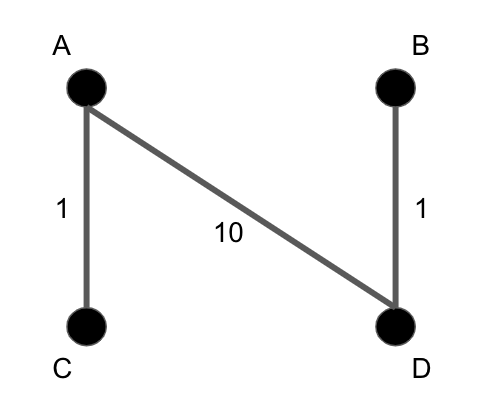
\includegraphics[width=2in]{4-1}

There are two ways to have a matching within $G$ here: one with $\{A, D \} \in M$ and one without. If $\{A, D \} \in M$ then the only way to increase the size of $M$ is to have some edge $\{ B, C\}$, which does not exist. So here, if we want to maximize $|M$, we find $|M| = 1$ and $w(M) = 10$.

Now suppose $\{A, D \} \notin M$. The other two edges in $E$ are $\{A, C \}$ and $\{B, D\}$, which have no nodes in common; therefore the maximal size of $M$ contains both of them. So here, trying to maximize $|M|$, we get $|M| = 2$ and $w(M) = 2$. 

So clearly the second case returns a larger $|M|$; however, the first case has a larger $w(M)$. Therefore there is no matching $M$ on $G$ that maximizes $w(M)$ and $|M|$, as desired.
\end{proof}

    \item (optional\footnotemark[1])
  
    One real-life constraint in kidney exchange is that donors $d$ are often associated with a particular patient $p$ (e.g. a close family member) such that $d$ is only willing to donate a kidney if $p$ receives a kidney from someone.  ($d$ would donate their kidney directly to $p$ if they could, but they are incompatible.) 
    Suppose we have an (unweighted) bipartite graph $G=(V_0\cup V_1,E)$ representing $n$ such donor-patient pairs, i.e. $V_0=\{d_0,d_1,\ldots,d_{n-1}\}$, $V_1 = \{p_0,p_1,\ldots,p_{n-1}\}$, where $p_i$ is the patient associated with donor $d_i$. We assume $\{d_i,p_i\}\notin E$ for each $i$.   Our goal is to find a matching $M$ of the largest possible size $|M|$, subject to the constraint that $d_i$ is matched in $M$ only if $p_i$ is matched in $M$. 

    Show that we can reduce this constrained version of the maximum matching problem to finding a maximum-weight {\em perfect} matching in an appropriate edge-weighted bipartite graph, where
    a perfect matching is a matching that matches all the vertices in the graph. (Hint: add edges $\{d_i,p_i\}$ with appropriate edge weights.) 

\begin{proof}

\end{proof}

    \end{enumerate}
    

\end{enumerate}
\end{document}
